\documentclass[12pt,a4paper]{article}

% ── Packages ──────────────────────────────────────────────────────────────────
\usepackage[T1]{fontenc}
\usepackage[utf8]{inputenc}
\usepackage{lmodern}
\usepackage[british]{babel}
\usepackage{geometry}
\geometry{margin=2.5cm}
\usepackage{setspace}
\onehalfspacing
\usepackage{parskip}
\usepackage{graphicx}
\graphicspath{{figures/}}
\usepackage{float}
\usepackage{booktabs}
\usepackage{longtable}
\usepackage{array}
\usepackage{tabularx}
\usepackage{multirow}
\usepackage{caption}
\usepackage{hyperref}
\hypersetup{colorlinks=true, linkcolor=black, citecolor=black, urlcolor=blue}
\usepackage{natbib}
\bibliographystyle{apalike}
\usepackage{titlesec}
\usepackage{xcolor}
\usepackage{fancyhdr}
\usepackage{amsmath}
\usepackage{microtype}
\usepackage{pdflscape}
\usepackage{rotating}
\usepackage{seqsplit}

% ── Header / footer ───────────────────────────────────────────────────────────
\pagestyle{fancy}
\fancyhf{}
\rhead{Coffee Suitability on Hawai\okina i}
\lhead{DAM and Flowchart}
\cfoot{\thepage}

% ── Custom okina character ─────────────────────────────────────────────────────
\newcommand{\okina}{\textquoteleft}

% ── Breakable filename helper (allows wrapping at underscores) ─────────────────
\newcommand{\fn}[1]{\seqsplit{#1}}

% ══════════════════════════════════════════════════════════════════════════════
\begin{document}
% ══════════════════════════════════════════════════════════════════════════════

% ── Title block ───────────────────────────────────────────────────────────────
\begin{center}
  {\LARGE\bfseries Data Action Model and Flowchart\par}
  \vspace{0.4em}
  {\large Coffee Bean Production Suitability on Hawai\okina i\par}
  \vspace{0.8em}
  {\normalsize Geo-information Science and Remote Sensing\\
  Data Acquisition and Management: Group Project\par}
  \vspace{0.6em}
  {\small Ella Jansma (s1114516), Max Claessens (s1097783), Gijs Bomert (s1117543),\\
  Jochem Oude Groeniger (s1141308), Pieterjan Pauwelyn (s1089656)\par}
\end{center}

\vspace{1em}

% ── Intro paragraph ───────────────────────────────────────────────────────────
In this document the Data Action Model (DAM) is presented in the form of a flowchart that visually outlines all analysis steps undertaken in this project (Figure~\ref{fig:dam}). The flowchart provides a structured overview of the workflow, from data acquisition and preprocessing through transformation and analysis to the final suitability modelling. Each step represents a specific GIS operation applied to the datasets, ensuring transparency and reproducibility of the methodology. Below the flowchart, a detailed action table (Table~\ref{tab:dam_actions}) describes every individual step, including the type of data handling, the operation performed, and the objective of each action. A dataset table (Table~\ref{tab:dam_intermediate}) then describes the input datasets and the intermediate results they produce.

% ── Flowchart ─────────────────────────────────────────────────────────────────
\begin{figure}[H]
  \centering
  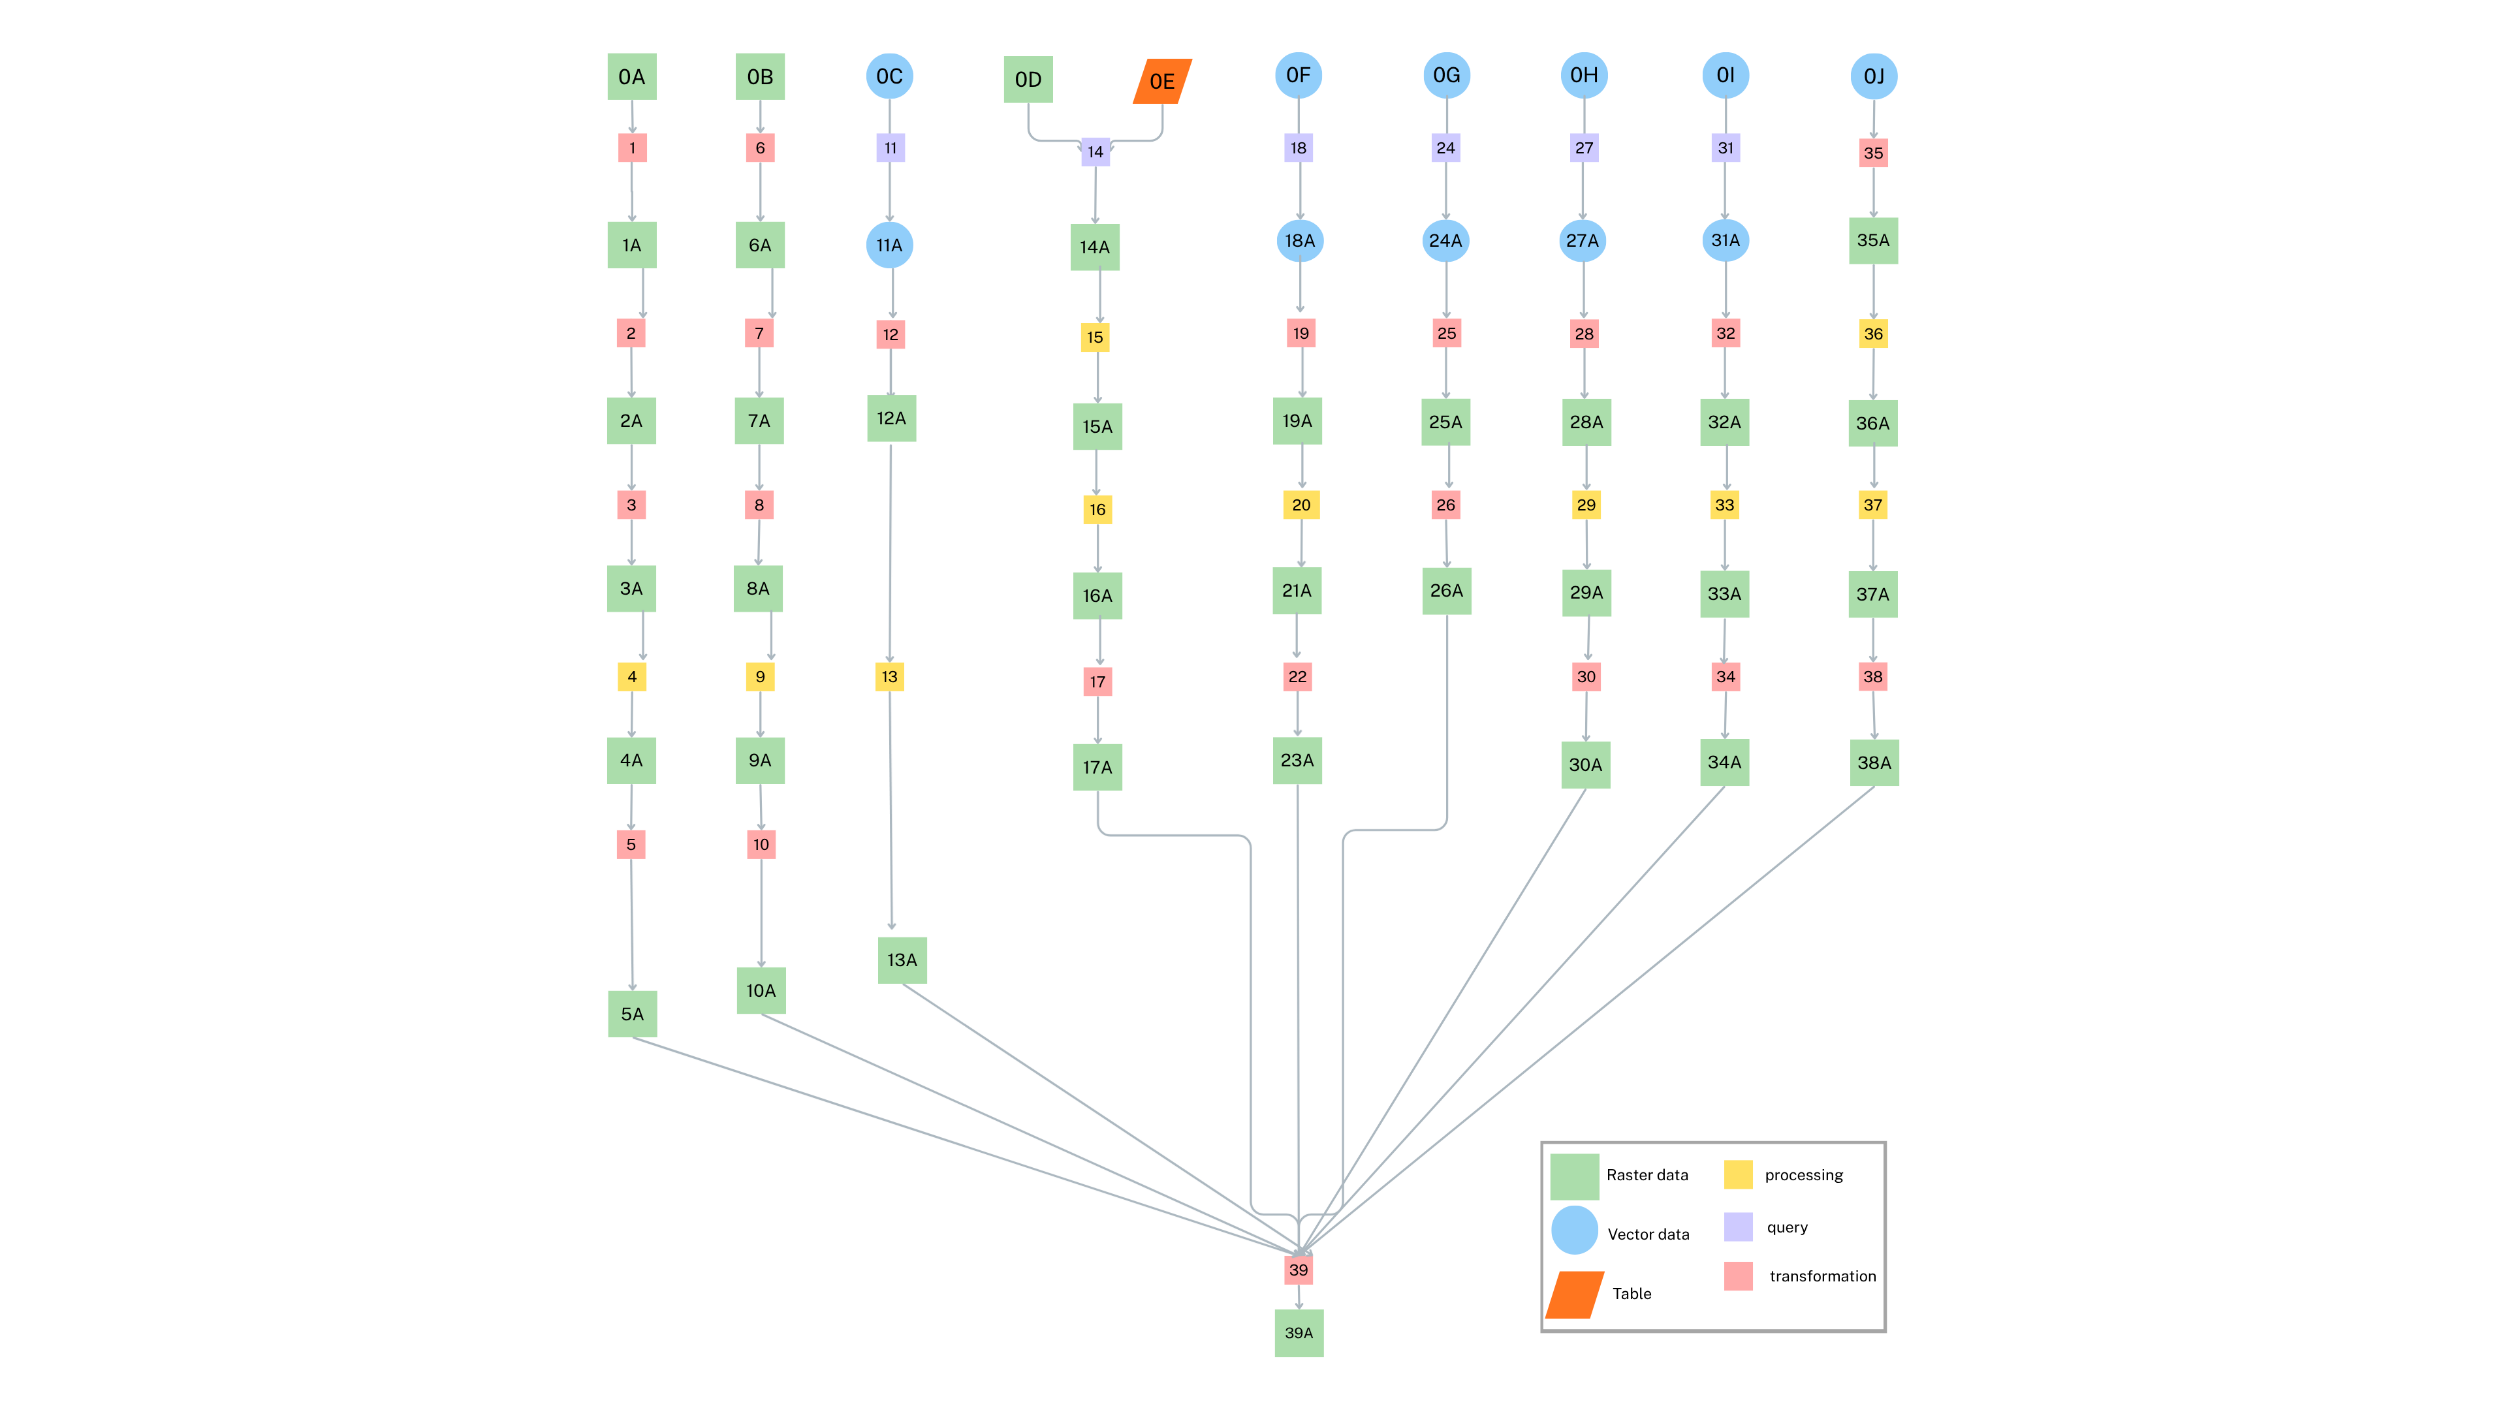
\includegraphics[width=\textwidth]{dam_flowchart.png}
  \caption{Data Action Model showing the steps of the analysis. See Tables~\ref{tab:dam_actions} and~\ref{tab:dam_intermediate} for an explanation of the steps and intermediate results.}
  \label{fig:dam}
\end{figure}

% ── Table 1: Action description ───────────────────────────────────────────────
\begin{landscape}
\begin{longtable}{@{}c >{\raggedright\arraybackslash}p{2.4cm} >{\raggedright\arraybackslash}p{4.2cm} >{\raggedright\arraybackslash}p{9.1cm}@{}}
  \caption{Action description table describing all analysis actions.}
  \label{tab:dam_actions}\\
  \toprule
  \textbf{Action} & \textbf{Type of handling} & \textbf{Operation} & \textbf{Objective} \\
  \midrule
  \endfirsthead
  \multicolumn{4}{c}{\itshape (Table~\ref{tab:dam_actions} continued)}\\
  \toprule
  \textbf{Action} & \textbf{Type of handling} & \textbf{Operation} & \textbf{Objective} \\
  \midrule
  \endhead
  \bottomrule
  \endfoot
  % ─── PRECIPITATION ───────────────────────────────────────────────────────────
  \multicolumn{4}{@{}l}{\textit{\textbf{Precipitation} (for all three projections)}} \\
  \addlinespace
  1 & Transformation & Clip Raster & Restrict the rasters (current precipitation + SSP1-2.6 + SSP3-7.0 + SSP5-8.5) to the Hawai\okina i study area to remove irrelevant data. \\
  2 & Transformation & Project Raster (if needed); Resample; Set Snap Raster & Ensure all rasters share the same CRS, spatial resolution, and alignment as the common raster framework. \\
  3 & Transformation & Unit check and conversion (Raster Calculator if needed) & Convert monthly values (mm/month) to annual precipitation (mm/year). Range for 3-tier suitability scoring: $<$1{,}100\,mm (score 1); 1{,}100--1{,}600\,mm or 1{,}800--2{,}000\,mm (score 2); 1{,}600--1{,}800\,mm (score 3); $>$2{,}000\,mm (score 1). Thresholds adapted from \citet{DaMatta2006}. \\
  4 & Processing & Reclassify Raster & Reclassify the annual precipitation raster to 3-tier suitability scores on a 1--3 scale: $<$1{,}100\,mm/year $\rightarrow$ 1 (unsuitable); 1{,}100--1{,}600\,mm/year $\rightarrow$ 2 (suboptimal); 1{,}600--1{,}800\,mm/year $\rightarrow$ 3 (optimal); 1{,}800--2{,}000\,mm/year $\rightarrow$ 2 (suboptimal); $>$2{,}000\,mm/year $\rightarrow$ 1 (unsuitable). \\
  5 & Transformation & Copy Raster / Export Raster (separate outputs per dataset) & Store each precipitation suitability raster separately to enable later comparison and overlay analysis. \\
  \addlinespace
  % ─── TEMPERATURE ─────────────────────────────────────────────────────────────
  \multicolumn{4}{@{}l}{\textit{\textbf{Temperature} (for all three projections)}} \\
  \addlinespace
  6 & Transformation & Clip Raster & Restrict the rasters (current temperature + SSP1-2.6 + SSP3-7.0 + SSP5-8.5) to the Hawai\okina i study area to remove irrelevant data and ensure spatial consistency. \\
  7 & Transformation & Project Raster (if needed); Resample; Set Snap Raster & Ensure all rasters share the same CRS, spatial resolution, and alignment as the common raster framework. \\
  8 & Transformation & Unit check and conversion (Raster Calculator if needed) & Convert tenths of °C (°C $\times$ 10) to degrees Celsius if needed. Target range for 3-tier suitability scoring: $<$15\,°C (score 1); 15--18\,°C or 23--26\,°C (score 2); 18--23\,°C (score 3); $>$26\,°C (score 1). \\
  9 & Processing & Reclassify Raster & Reclassify the temperature raster to 3-tier suitability scores on a 1--3 scale: $<$15\,°C $\rightarrow$ 1 (unsuitable); 15--18\,°C $\rightarrow$ 2 (suboptimal); 18--23\,°C $\rightarrow$ 3 (optimal); 23--26\,°C $\rightarrow$ 2 (suboptimal); $>$26\,°C $\rightarrow$ 1 (unsuitable). \\
  10 & Transformation & Copy Raster / Export Raster (separate outputs per dataset) & Store each temperature suitability raster separately to enable later comparison and overlay analysis. \\
  \addlinespace
  % ─── ROADS ───────────────────────────────────────────────────────────────────
  \multicolumn{4}{@{}l}{\textit{\textbf{Roads}}} \\
  \addlinespace
  11 & Selection & Select Layer By Attribute & Filter Roads\_-\_Hawaii\_County to retain only roads of class A35, A31, or Q05, removing local roads and leaving only those relevant to the analysis. \\
  12 & Transformation & Distance Accumulation & Create a raster dataset in which each cell value is the distance to the nearest usable road. \\
  13 & Processing & Reclassify & Create a 3-tier suitability score: $<$2{,}000\,m $\rightarrow$ optimal (3); 2{,}000--5{,}000\,m $\rightarrow$ suboptimal (2); $>$5{,}000\,m $\rightarrow$ unsuitable (1). \\
  \addlinespace
  % ─── SOIL TYPE ───────────────────────────────────────────────────────────────
  \multicolumn{4}{@{}l}{\textit{\textbf{Soil type}}} \\
  \addlinespace
  14 & Query (thematic) & Join (value field = Number) & Join the raster TAXOUSDA\_250m\_ll.tif with the table TAXOUSDA\_250m\_ll.tif.csv to link the numeric raster values to generic soil type names in the table. \\
  15 & Processing by overlay & Clip Raster & Clip the raster to the main island of Hawai\okina i, removing all other areas. \\
  16 & Processing & Reclassify Raster & Convert generic soil types to suitability scores: Andisols, Ultisols, Inceptisols $\rightarrow$ 3 (optimal); other orders $\rightarrow$ 2 (suboptimal); Aridisols, Histosols $\rightarrow$ 1 (unsuitable). \\
  17 & Transformation & Copy Raster / Export Raster & Store the soil type suitability raster to enable later comparison and overlay analysis. \\
  \addlinespace
  % ─── LAND USE, CONSERVATION AND TERRAIN ──────────────────────────────────────
  \multicolumn{4}{@{}l}{\textit{\textbf{Land use, conservation, and terrain}}} \\
  \addlinespace
  18 & Query (thematic) & Select by Attribute & In dataset 0F, select records present on Hawai\okina i and clip the dataset. \\
  19 & Transformation & Polygon to Raster & Convert the conservation district data for Hawai\okina i into a raster. \\
  20 & Processing & Reclassify Raster & Convert to suitability scores: G (General), C (Undesignated) $\rightarrow$ 1 (suitable); R (Resource) $\rightarrow$ 0.75; L (Limited) $\rightarrow$ 0.25; P (Protective), SS (Special subzone) $\rightarrow$ 0 (unsuitable). \\
  21 & Transformation & Export Raster & Store the conservation district raster to enable later comparison and overlay analysis. \\
  22 & Query (thematic) & Select by Attribute & In dataset 0G, select records present on Hawai\okina i. \\
  23 & Transformation & Polygon to Raster & Convert the critical habitat data for Hawai\okina i into a raster. \\
  24 & Transformation & Export Raster & Store the critical habitat raster to enable later comparison and overlay analysis. The suitability score of 0 is already included in the unmodified dataset. \\
  25 & Query (thematic) & Select by Attribute & In dataset 0H, select records present on Hawai\okina i and clip the dataset. \\
  26 & Transformation & Polygon to Raster & Convert the Department of Defense data for Hawai\okina i into a raster. \\
  27 & Processing & Reclassify Raster & Convert to suitability scores: military land $\rightarrow$ 0 (unsuitable). \\
  28 & Transformation & Export Raster & Store the Department of Defense raster to enable later comparison and overlay analysis. \\
  29 & Query (thematic) & Select by Attribute & In dataset 0I, select records present on Hawai\okina i and clip the dataset. \\
  30 & Transformation & Polygon to Raster & Convert the land use / land cover data for Hawai\okina i into a raster. \\
  31 & Processing & Reclassify Raster & Convert to suitability scores: classes 1\textasciitilde, 5\textasciitilde, 7\textasciitilde, 8\textasciitilde, 9\textasciitilde~$\rightarrow$ 0 (unsuitable); 2\textasciitilde, 3\textasciitilde~$\rightarrow$ 1 (suitable); 4\textasciitilde, 6\textasciitilde~$\rightarrow$ 0.5 (not preferred). \\
  32 & Transformation & Export Raster & Store the land use / land cover raster to enable later comparison and overlay analysis. \\
  \addlinespace
  % ─── ELEVATION ───────────────────────────────────────────────────────────────
  \multicolumn{4}{@{}l}{\textit{\textbf{Elevation}}} \\
  \addlinespace
  33 & Transformation & Topo to Raster & Convert the given polyline (contour) dataset into a usable raster. \\
  34 & Processing & Raster Calculator & Remove all negative elevation gradients (ocean floor). \\
  35 & Processing & Raster Calculator & Reclassify the elevation raster to 3-tier suitability scores on a 1--3 scale: $<$900\,m $\rightarrow$ 1 (unsuitable); 900--1{,}400\,m $\rightarrow$ 2 (suboptimal); 1{,}400--1{,}800\,m $\rightarrow$ 3 (optimal); 1{,}800--2{,}500\,m $\rightarrow$ 2 (suboptimal); $>$2{,}500\,m $\rightarrow$ 1 (unsuitable). \\
  36 & Transformation & Copy Raster / Export Raster & Store the elevation suitability raster for later comparison and overlay analysis. \\
  \addlinespace
  % ─── SUITABILITY MODELLING ───────────────────────────────────────────────────
  \multicolumn{4}{@{}l}{\textit{\textbf{Suitability modelling} (all projections)}} \\
  \addlinespace
  37 & Processing & Suitability Modeler & Combine temperature and precipitation suitability into the climate sub-model and store it for use in action 38. \\
  38 & Processing & Suitability Modeler & Combine the climate sub-model with the elevation, road, soil, conservation, critical habitat, Department of Defense, and land use / land cover layers to produce and store the final suitability raster for each projection. \\
\end{longtable}
\end{landscape}

% ── Table 2: Dataset description ──────────────────────────────────────────────
\begin{landscape}
\begin{longtable}{@{}l >{\raggedright\arraybackslash}p{4.2cm} >{\raggedright\arraybackslash}p{2.2cm} >{\raggedright\arraybackslash}p{2.4cm} >{\raggedright\arraybackslash}p{6.0cm} >{\raggedright\arraybackslash}p{1.9cm}@{}}
  \caption{Data description table of the data used for the analysis.}
  \label{tab:dam_intermediate}\\
  \toprule
  \textbf{ID} & \textbf{Dataset} & \textbf{Attribute} & \textbf{Meas. scale} & \textbf{Attribute domain} & \textbf{Data structure} \\
  \midrule
  \endfirsthead
  \multicolumn{6}{c}{\itshape (Table~\ref{tab:dam_intermediate} continued)}\\
  \toprule
  \textbf{ID} & \textbf{Dataset} & \textbf{Attribute} & \textbf{Meas. scale} & \textbf{Attribute domain} & \textbf{Data structure} \\
  \midrule
  \endhead
  \bottomrule
  \endfoot
  % Input datasets
  0A & Assignment data & Precipitation (mm/month) & Ratio & 0--$\infty$ & Raster \\
  0B & Assignment data & Temperature (°C) & Interval & $-\infty$--$\infty$ & Raster \\
  0C & \fn{Roads\_-\_Hawaii\_County} & Roads & Nominal & All & Vector \\
  0D & \fn{TAXOUSDA\_250m\_ll.tif} & Value & Nominal & 1--99 & Raster \\
  0E & \fn{TAXOUSDA\_250m\_ll.tif.csv} & Generic & Nominal & All & Table \\
  0F & Conservation District Subzones & Conservation District Code & Nominal & All & Vector \\
  0G & Areas of Critical Habitat (Consolidated) & Critical Habitats & Nominal & All & Vector \\
  0H & Department of Defense Lands & Base\_Name & Nominal & All & Vector \\
  0I & Land Use Land Cover (LULC) & LandCover & Nominal & 1--92 & Vector \\
  0J & \fn{Hawaii\_100\_Foot\_Contours} & Elevation & Ratio & 100--13{,}700\,ft & Vector \\
  \addlinespace
  % Precipitation intermediates
  1A & Clipped precipitation & Precipitation (mm/month) & Ratio & 0--$\infty$ & Raster \\
  2A & Aligned precipitation & Precipitation (mm/month) & Ratio & 0--$\infty$ & Raster \\
  3A & Annual precipitation & Precipitation (mm/year) & Ratio & 0--$\infty$ & Raster \\
  4A & Precipitation suitability & Precipitation (mm/year) & Ordinal & 1 (unsuit.: $<$1{,}100 or $>$2{,}000\,mm); 2 (subopt.: 1{,}100--1{,}600 or 1{,}800--2{,}000\,mm); 3 (opt.: 1{,}600--1{,}800\,mm) & Raster \\
  5A & Precipitation suitability (exported) & Precipitation (mm/year) & Ordinal & As 4A & Raster \\
  \addlinespace
  % Temperature intermediates
  6A & Clipped temperature & Temperature (°C) & Interval & $-\infty$--$\infty$ & Raster \\
  7A & Aligned temperature & Temperature (°C) & Interval & $-\infty$--$\infty$ & Raster \\
  8A & Converted temperature & Temperature (°C) & Interval & $-\infty$--$\infty$ & Raster \\
  9A & Temperature suitability & Temperature (°C) & Ordinal & 1 (unsuit.: $<$15 or $>$26\,°C); 2 (subopt.: 15--18 or 23--26\,°C); 3 (opt.: 18--23\,°C) & Raster \\
  10A & Temperature suitability (exported) & Temperature (°C) & Ordinal & As 9A & Raster \\
  \addlinespace
  % Roads
  11A & \fn{Highways\_Hawaii} & Roads & Binary & 1 (HWY, HIGHWAY) & Vector \\
  12A & Distance from roads & Roads & Ratio & 0--$\infty$\,m & Raster \\
  13A & Road suitability & Roads & Ordinal & 1 (unsuitable); 2 (suboptimal); 3 (optimal) & Raster \\
  \addlinespace
  % Soil
  14A & \fn{TAXOUSDA\_250m\_ll} (joined) & Generic & Nominal & All & Raster \\
  15A & \fn{TAXOUSDA\_250m\_ll\_Clip} & Generic & Nominal & All & Raster \\
  16A & \fn{Reclass\_TAXClip} & Generic & Ordinal & 1 (Aridisols, Histosols); 2 (other orders); 3 (Andisols, Ultisols, Inceptisols) & Raster \\
  17A & \fn{Reclass\_TAXClip} (exported) & Generic & Ordinal & As 16A & Raster \\
  \addlinespace
  % Conservation
  18A & \fn{Conservation\_Districts\_Hawaii} & Terrain & Nominal & G, C, R, L, P, SS & Vector \\
  19A & \fn{CD\_Hawaii\_Raster} & Terrain & Nominal & G, C, R, L, P, SS & Raster \\
  20A & \fn{CD\_Suitability} & Terrain & Categorical & 1 (G, C); 0.75 (R); 0.25 (L); 0 (P, SS) & Raster \\
  21A & \fn{CD\_Suitability} (exported) & Terrain & Categorical & As 20A & Raster \\
  \addlinespace
  % Critical habitat
  22A & \fn{Critical\_Habitat\_Hawai}\okina i & Conservation & Categorical & 0 (critical habitat) & Vector \\
  23A & CHR & Conservation & Categorical & 0 (critical habitat) & Raster \\
  24A & CHR (exported) & Conservation & Categorical & 0 (critical habitat) & Raster \\
  \addlinespace
  % DoD
  25A & \fn{DeptofDefense\_Hawaii} & Land use & Nominal & Base\_Name & Vector \\
  26A & DDR & Land use & Nominal & Base\_Name & Raster \\
  27A & ArmyArea & Land use & Categorical & 0 (military land) & Raster \\
  28A & ArmyArea (exported) & Land use & Categorical & 0 (military land) & Raster \\
  \addlinespace
  % LULC
  29A & LandUseLandCover & Land use & Nominal & 1\textasciitilde~(Urban); 2\textasciitilde~(Agriculture); 3\textasciitilde~(Rangeland); 4\textasciitilde~(Forest); 5\textasciitilde~(Water); 6\textasciitilde~(Wetland); 7\textasciitilde~(Barren); 8\textasciitilde~(Tundra); 9\textasciitilde~(Perm. snow) & Vector \\
  30A & USLUR & Land use & Nominal & As 29A & Raster \\
  31A & LandUseSuitability & Land use & Categorical & 0 (1\textasciitilde,5\textasciitilde,7\textasciitilde,8\textasciitilde,9\textasciitilde); 0.5 (4\textasciitilde,6\textasciitilde); 1 (2\textasciitilde,3\textasciitilde) & Raster \\
  32A & LandUseSuitability (exported) & Land use & Categorical & As 31A & Raster \\
  \addlinespace
  % Elevation
  33A & Elevation raster & Elevation & Ratio & $-$2{,}562--13{,}493\,ft & Raster \\
  34A & Positive elevation raster & Elevation & Ratio & 0--13{,}493\,ft & Raster \\
  35A & Elevation suitability & Elevation & Ordinal & 1 (unsuit.: $<$900 or $>$2{,}500\,m); 2 (subopt.: 900--1{,}400 or 1{,}800--2{,}500\,m); 3 (opt.: 1{,}400--1{,}800\,m) & Raster \\
  36A & Elevation suitability (exported) & Elevation & Ordinal & As 35A & Raster \\
  \addlinespace
  % Final outputs
  37A & Climate sub-model (per scenario) & Climate suitability & Ratio & n/a & Raster \\
  38A & Coffee Plantation Suitability & Suitability model & Ratio & n/a & Raster \\
\end{longtable}
\end{landscape}

% ── References (for the DaMatta2006 citation in the action table) ─────────────
\bibliography{references}

\end{document}
